\documentclass[reprint, nofootinbib, nobalancelastpage, 10pt]{revtex4-2}

\usepackage[T2A]{fontenc}			% кодировка
\usepackage[utf8]{inputenc}			% кодировка исходного текста
\usepackage[english,russian]{babel}	% локализация и переносы

\usepackage{amsmath,amsfonts,amssymb,amsthm,bm,mathtools}

\usepackage[usenames]{color}
\usepackage{colortbl}
\usepackage{indentfirst} %Красная строка
\usepackage{hyperref}

\usepackage{booktabs}
\usepackage{graphicx}  % Для вставки рисунков
\graphicspath{{images/}{graphs/}}  % папки с картинками

\renewcommand*{\thefootnote}{\alph{footnote}}

\begin{document}

\title{Электронный парамагнитный резонанс}
\author{Илларионов Владислав}
\affiliation{группа Б04-855}

\maketitle


\section*{Введение}

В ходе данной работы исследуется электронной парамагнитный резонанс в молекуле ДФПГ,
определяется $g$-фактор электрона и из анализа пика сигнала ЭПР на осциллографе измеряется
ширина линии ЭПР.


\section*{Теоретическая часть}

Энергетический уровень электрона в присутствии магнитного поля с индукцией $B$
расщепляется на два подуровня, расстояние между которыми равно:
\begin{equation}
	\label{eq:epr}
	\Delta E = E_2 - E_1 = 2 \mu B = \hbar \omega_0
\end{equation}

Здесь $\mu$ --- абсолютная величина проекции магнитного момента на направление поля.
$\omega_0$ --- резонансная частота внешнего электромагнитного поля.

Возбуждение электронных резонансных переходов электромагнитным полем, имеющим частоту,
определяемую формулой~(\ref{eq:epr}), носит название электронного парамагнитного
резонанса (ЭПР). ЭПР возникает из-за переворота спина электронов под действием
высокочастотного электромагнитного поля. Однако переворот спинов возможен только у
неспаренных электронов, наличие которых как раз и приводит к парамагнетизму.

Структурная формула свободного радикала ДФПГ, который исследуется в данной работе,
представлена на рисунке~\ref{img:1}.

\begin{figure}[h!]
	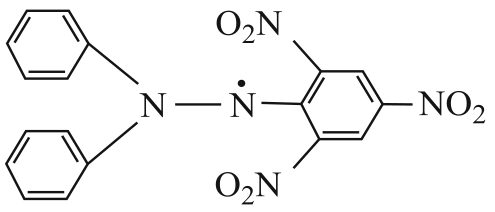
\includegraphics[width=0.6\linewidth]{1.png}
	\caption{Структурная формула молекулы ДФПГ}
	\label{img:1}
\end{figure}

Связь между магнитным моментом $\bm{\mu}$ электрона и его механическим моментом
$\mathbf{M}$ выражается через гиромагнитное отношение $\gamma$ с помощью формулы:
\begin{equation}
	\bm{\mu} = \gamma \mathbf{M}
\end{equation}

Если выражать магнитный момент в магнетонах бора $\mathfrak{m}_{\text{Б}}$, а механический
в единицах $\hbar$, то:
\begin{equation}
	\dfrac{\bm{\mu}}{\mathfrak{m}_{\text{Б}} } = \dfrac{g \mathbf{M}}{\hbar}
\end{equation}

$g$-фактор можно выразить через величины определяемые экспериментально:
\begin{equation}
	g = \dfrac{\hbar \omega_0}{\mathfrak{m}_{\text{Б}} B}
\end{equation}

Чисто спиновый характер магнетизма в ДФПГ приводит к тому, что парамагнитный резонанс
на неспаренных электронах происходит почти как на свободных частицах. Поэтому $g$-фактор,
полученный из электронного парамагнитного резонанса в ДФПГ, всего на десятые доли процента
отличается от $g$-фактора свободного электрона.

Рассмотрим основные процессы, влияющие на ширину линии ЭПР. В отсутствие высокочастотного
поля заселенность верхнего и нижнего уровней описывается обычной формулой Больцмана.
В присутствии резонансного поля между уровнями возникают индукционные переходы, ведущие к
тому, что заселенность верхнего уровня растет, а нижнего --- падает.

Восстановление теплового равновесия в заселенностях уровней осуществляется за счет
передачи энергии возбуждения другим степеням свободы тела. Передача энергии в другие
степени свободы осуществляется за счет спин-спинового и спин-решеточного взаимодействий.

Оба типа взаимодействия способствуют релаксации и, следовательно, укорачивают время,
которое проводит электрон на верхнем уровне. Ширина уровня связана с временем релаксации
соотношением неопределенностей:
\begin{equation}
	\Delta E \simeq \dfrac{\hbar}{\tau} \Longrightarrow \Delta \omega \simeq \tau^{-1}
\end{equation}


\section*{Экспериментальная установка}

\begin{figure}[h!]
	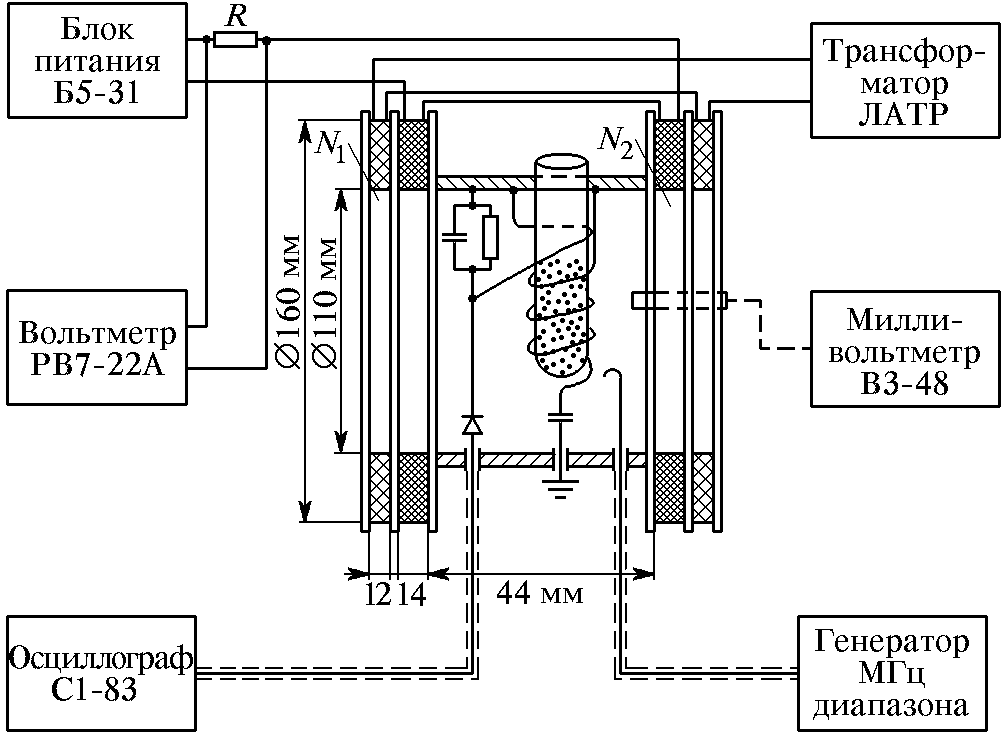
\includegraphics[width=0.6\linewidth]{2.png}
	\caption{Блок-схема установки}
	\label{img:2}
\end{figure}

В данной работе используется радиоспектроскоп, работающий в диапазоне 100-200 МГц.
Его действие основно на уменьшении добротности контура при появлении резонансных
парамагнитных потерь. Схема радиоспектроскопа изображена на рисунке~\ref{img:2}.
Основной частью радиоспектроскопа является колебательный контур. Он состоит из катушек
индуктивности и плоского конденсатора. Ампула с исследуемым образцом вставляется в катушку
индуктивности контура. Основное магнитное поле в образце создается с помощью двух соосно
расположенных катушек, питаемых от источника постоянного тока. Величина тока, протекающего
через катушки, регулируется ручкой, расположенной на блоке питания, и измеряется с помощью
вольтметра и омического сопротивления. Небольшое модулирующее поле создается при помощи
дополнительных катушек. Они включены в сеть переменного тока через трансформатор.

Электромагнитные колебания в контуре возбуждаются генератором радиочастотного диапазона.
Связь с генератором осуществляется с помощью петли. Через полупроводниковый диод контур
подключен к вертикальному усилителю осциллографа. Колебательный контур соединен с
генератором и осциллографом коаксиальным кабелем.

Параметры основных катушек установки:
\begin{eqnarray*}
	N_1 = 6700 \hspace*{1cm} d_1 = 0.25 \text{ м} \\
	N_2 = 5000 \hspace*{1cm} d_2 = 0.30 \text{ м}
\end{eqnarray*}

Параметры пробной катушки:
\[n = 45 \hspace{1cm} d = (15.2 \pm 1) \text{ мм}\]

\section*{Методика измерения}

Ампула с исследуемым веществом помещается внутрь катушки индуктивности радиоспектроскопа.
Настроим генератор на резонансную частоту колебательного контура. Детектирование усредняет
высокочастотный сигнал, а его огибающая превращается в низкочастотный переменный сигнал,
легко визуализируемый на осциллографе. Для наблюдения сигнала переведем осциллограф в
режим развёртки по времени. По изображению на осциллографе можно определить резонансное
значение частоты (соответствуют максимуму амплитуды). Настроив генератор на резонансную
частоту, переведем его на работу в режиме непрерывной генерации.

Плавно меняя реостатом величину тока, проходящего через основные катушки, найдем сигнал
ЭПР. Если основное поле $B$ подобрано точно, то на экране осциллографа сигналы ЭПР
располагаются через равные промежутки (см.~рис.~\ref{img:3}).

\begin{figure}[h!]
	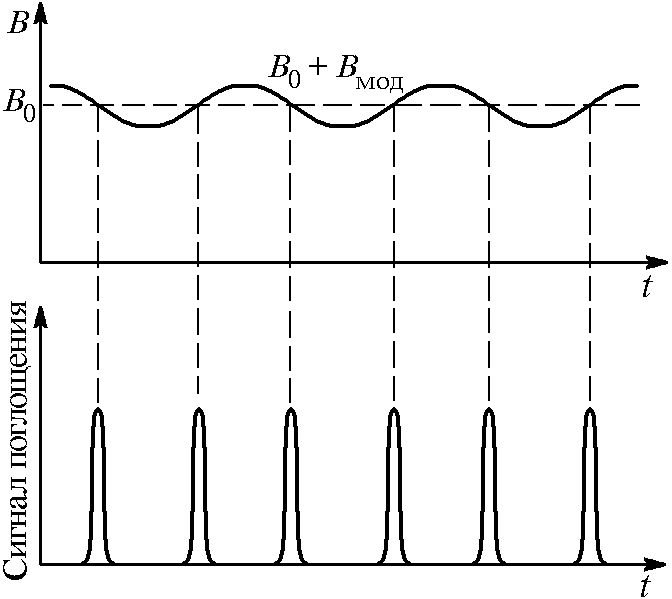
\includegraphics[width=0.8\linewidth]{3.png}
	\caption{Сигналы ЭПР на экране осциллографа, при точной настройке основного поля}
	\label{img:3}
\end{figure}

$g$-фактор электрона определяем следующим образом.

Будем измерять переменное поле, поэтому заметим показания вольтметра, измеряющего
постоянный ток в катушках, а затем переключим их на переменный ток, подобрав положения
движков автотрансформатора так, чтобы показание вольтметра было равно замеченному ранее
значению. Введем пробную катушку внутрь основных катушек поблизости от образца и снимем
показания лампового милливольтметра V. Зная число витков $n$ и площадь сечения $S$ пробной
катушки, определим величину магнитного поля из соотношения:
\begin{equation}
	\label{eq:B}
	V = n B_0 S \omega_{\simeq}
\end{equation}

Здесь $\omega_{\simeq} = (2 \pi \cdot 50 \text{ Гц})$ --- угловая частота переменного тока.

Для определения ширины линии ЭПР переключим осциллограф с временной развертки на развертку
от модуляционных катушек. Длина развертки будет соответствовать удвоенной амплитуде
модулирующего поля (см.~рис.~\ref{img:5}). Амплитуду этого поля определим из соотношения~(\ref{eq:B}) аналогичным
способом.

\begin{figure}[h!]
	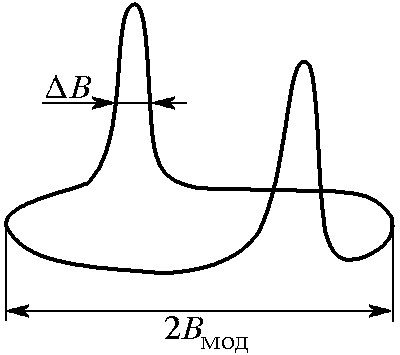
\includegraphics[width=0.5\linewidth]{5.png}
	\caption{Сигналы поглощения ЭПР при развертке луча осциллографа напряжением
				модулирующих катушек}
	\label{img:5}
\end{figure}

Тогда ширину линии ЭПР можно получить из соотношения:
\begin{equation}
	\Delta B = 2 \dfrac{A_{1/2}}{A_{\text{полн}}} B_{\text{мод}}
\end{equation}

Здесь $A_{1/2}$ --- количество делений полуширины на экране осциллографа,
$A_{\text{полн}}$ --- количество делений всей длины развертки.

\section*{Обработка данных}

\subsection{Измерение g-фактора электрона}

Сперва настраиваем генератор на резонансную частоту. Её значение (по лимбу генератора):
\[f_0 = (164 \pm 2) \text{ МГц}\]

Изменяя магнитное поле в катушках так, чтобы достичь одинакового расстояния между пиками
на осциллографе. Магнитное поле $B_0$ находим с помощью пробной катушки: запишем
напряжение $V = 15.68$ мВ на катушках при постоянном поле, заменим его на переменное с
таким же значением напряжения.
\[ B_0 = \dfrac{V}{n S \omega_{\simeq}} = (6.12 \pm 0.08) \text{ мТл} \]

Тогда $g$-фактор:
\[ g = \dfrac{\hbar \omega_0}{\mathfrak{m}_{\text{Б}} B_0} = 1.91 \pm 0.03 \]

\subsection{Определение ширины линии ЭПР}

Переключим осциллограф на развертку модулирующих катушек. Аналогично предыдущему пункту
определим действующее значение модулирующего поля:
\[ B_{\text{мод}} = \dfrac{V}{n S \omega_{\simeq}} = (0.79 \pm 0.01) \text{ мТл} \]

\begin{figure}[h!]
	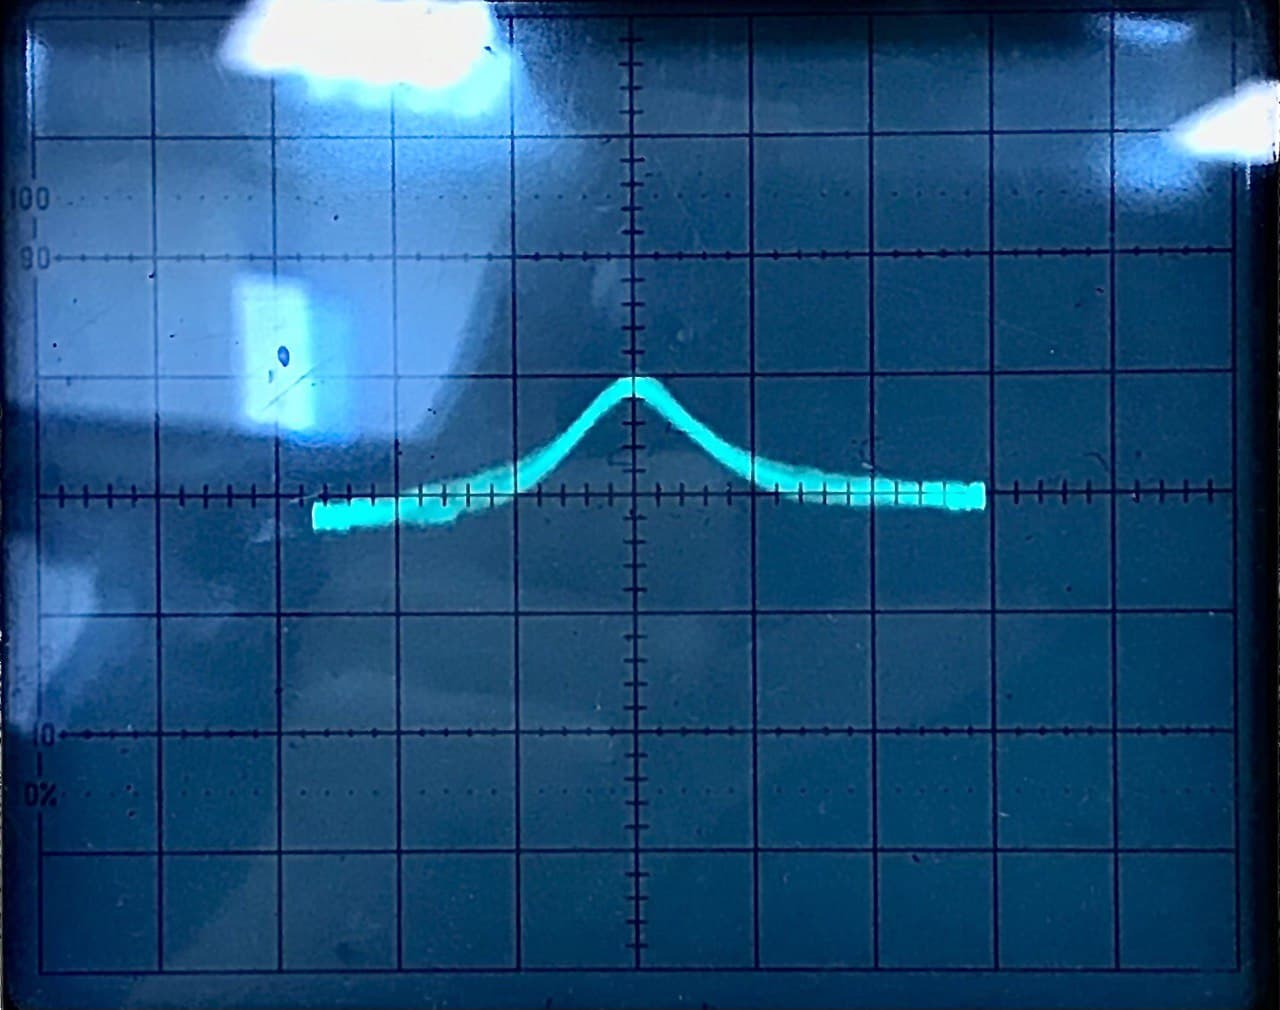
\includegraphics[width=0.8\linewidth]{4.png}
	\caption{Изображение на экране осциллографа при переключении на развертку
				модулирующих катушек}
	\label{img:4}
\end{figure}

По осциллографу (см.~рис.~\ref{img:4}):
\begin{eqnarray*}
	A_{1/2} &=& (0.8 \pm 0.1) \text{ дел} \\
	A_{\text{полн}} &=& (5.6 \pm 0.1) \text{ дел}
\end{eqnarray*}

Значит:
\[\Delta B = (0.226 \pm 0.036) \text{ мТл} = (2.26 \pm 0.36) \text{ Гс}\]

\section*{Вывод}

В ходе данной работы было исследовано явление электронного парамагнитного резонанса в
молекуле дифенилпикрилгидразила (ДФПГ). По $g$-фактору этой молекулы была получена оценка
$g$-фактора электрона:
\[ g = 1.91 \pm 0.03, \]

которая близка к теоретическому значению.

Также была найдена ширина линии ЭПР по осциллографу:
\[ \Delta B = (2.26 \pm 0.36) \text{ Гс} \]

\end{document}
